\section{Pre-Procesamiento}

    A continuación se describen las herramientas y métodos usados en el pre-procesamiento para obtener los datos del sensor Kinect, crear la nube de puntos,  y separar la nube de puntos en nubes mas pequeñas que contienen los objetos a representar.
   
    
    \subsection{Biblioteca de Nubes de Puntos(PCL)}
    
    	
        Para realizar el manejo de \glspl{nube de puntos} se uso la biblioteca de nubes de puntos (PCL por sus iniciales en inglés)\cite{Rusu_ICRA2011_PCL}, la cual cuenta con un conjunto de herramientas comúnmente usadas para quitar ruido, agrupar puntos, segmentación, etc.\\
        
        \begin{figure}[!htb] 
            \centering
            
\includegraphics[width=0.6\textwidth]{02Desarrollo/Preprocesamiento/imagenes/pointcloudlibrary_vert_large_pos.png}
            \caption{Logo de la Biblioteca de Nube de Puntos} 
            \label{fig:PCL}
        \end{figure}
        
        PCL es un proyecto de código abierto. El logotipo del proyecto se puede ver en la figura \ref{fig:PCL}, desarrollado y apoyado por grandes empresas, este proyecto se distribuye bajo la licencia BSD modificada (de 3 cláusulas). Se ha probado en sistemas Linux, MacOS y Windows, además de que el código esta creado de forma modular lo que permite elegir que características usar y cuales descartar.\\
        
        
    \subsection{Obtención de datos}
    
        La obtención de una nube de puntos puede ser dada por una variedad de \glspl{sensor}, estos se clasifican según la tecnología usada para obtener la imagen de profundidad, algunos ejemplos son los sensores: ultrasónicos, infrarrojos, estereoscópicos. En este caso particular se utiliza el sensor de Microsorft Kinect 2.0, ya que es uno de los dispositivos que generan imágenes de profundidad con mayor soporte y de los más conocidos, ademas con un precio de \$2,699.00 MXN \cite{XBOXONEK76:online}, es un dispositivo bastante accesible.\\
        
        Para generar la nube de puntos a usar es necesario un intermediario entre PCL y el Kinect ya que los datos del Kinect no se encuentran listos para ser usados directamente con la bibliotecas de PCL, ya que la información obtenida del Kinect son tres imágenes, de color, infrarroja y de profundidad,como se muestra en la figura \ref{fig:imgKinect} \cite{UsodelKi56:online}, estas imágenes se combinan para construir una nube de puntos, primero se juntan las imágenes de color y la de profundidad y luego se genera la nube de puntos la cual representa cada pixel de la imagen de profundidad en un arreglo de puntos junto con el color asignado a cada uno. \\
          
         \begin{figure}[!htb] 
         	\centering
         	\subfloat[
         	\label{fig:color}]{%
         		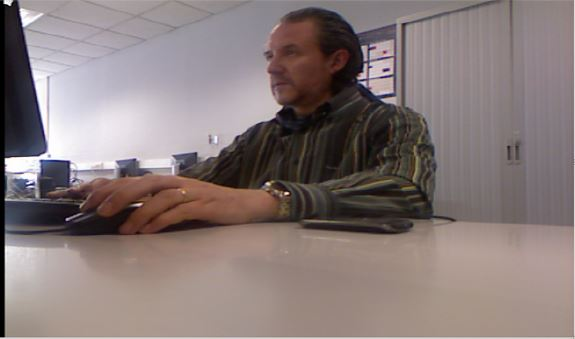
\includegraphics[width=0.33\textwidth]{02Desarrollo/Preprocesamiento/imagenes/color.jpg}
         	}
         	\subfloat[
         	\label{fig:ir}]{%
         		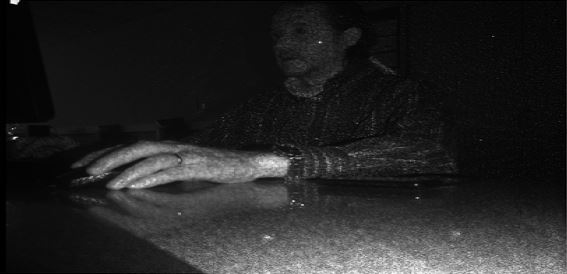
\includegraphics[width=0.33\textwidth]{02Desarrollo/Preprocesamiento/imagenes/ir.jpg}
         	}
         	\subfloat[
         	\label{fig:profundidad}]{%
         		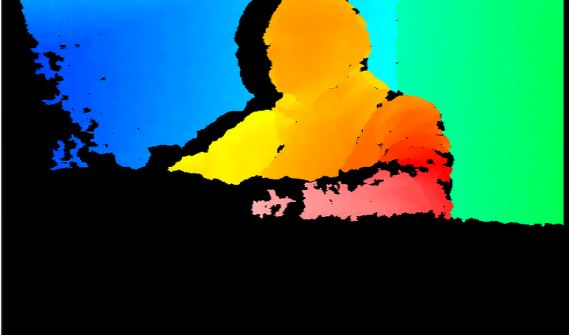
\includegraphics[width=0.33\textwidth]{02Desarrollo/Preprocesamiento/imagenes/profundidad.jpg}
         	}
         
         	\caption[Datos obtenidos del dispositivo Kinect.]{Datos obtenidos del dispositivo Kinect, (a) Imagen de la cámara a color, (b)Imagen de la cámara infrarroja, (c)Imagen de profundidad.} 
         	\label{fig:imgKinect}
         \end{figure}
         
        El \gls{controlador} libfreenect \cite{libfreenect} se comunica con el Kinect y obtiene las imágenes a color RGB, infrarrojas (IR) y profundidad. Este proyecto fue el resultado. del trabajo de H. Martín para el concurso que
        lanza Adafruit \cite{UsodelKi56:online} \\ 
        
        
       
        
        Mientras libfreenect2pclgrabber \cite{k2g} es un proyecto desarrollado por  Dr. Giacomo Dabisias ingeniero de software en lyft \cite{k2g},  que cuenta con una biblioteca que actúa como intermediario creando nubes de puntos a partir de las imágenes  infrarrojas, de profundidad y color obtenidas del controlador libfreenect. Se uso este proyecto de software libre ya que cuenta con soporte para sistemas operativos Linux, MacOs y Windows, permitiendo la reproducción e integración del sistema desarrollado en diferentes sistemas operativos.  \\ 
        
        Luego de que el controlador obtiene los datos del sensor y son convertidos en una nube de puntos es posible empezar a trabajar con ellos usando las herramientas de PCL.\\
    
    \subsection{Filtrado de densidad de puntos}
    
        Dado que la nube de puntos obtenida cuenta con muchos datos, el procesamiento se vuelve lento. Para disminuir la carga de trabajo de la computadora lo primero que se realiza es un filtrado de densidad de puntos, dicho de otra manera se busca disminuir la cantidad de puntos en la nube, parecido a cuando se reduce el tamaño de una imagen.\\
        
        Este \gls{filtro} calcula una nueva nube de puntos la cual contiene menos información de la original, un ejemplo de este filtro se puede ver en la figura \ref{fig:FiltroDensidad}. cada uno de los nuevos puntos es una representación de un conjunto de puntos que se encuentran dentro de alguna vecindad.\\
        
        Los pasos para este filtro son:
        \begin{itemize}
            \item El filtro divide la nube de puntos en un arreglo de cubos.
            \item Luego se calcula el centroide de cada división usando todos los puntos que se encuentran dentro de esta.
            \item Al final se crea una nueva nube de puntos usando los centroides obtenidos.
        \end{itemize}
        
        
        
        
        \begin{figure}[!htb] 
        	\centering
        	\subfloat[
        	\label{fig:FiltroDensidadA}]{%
        		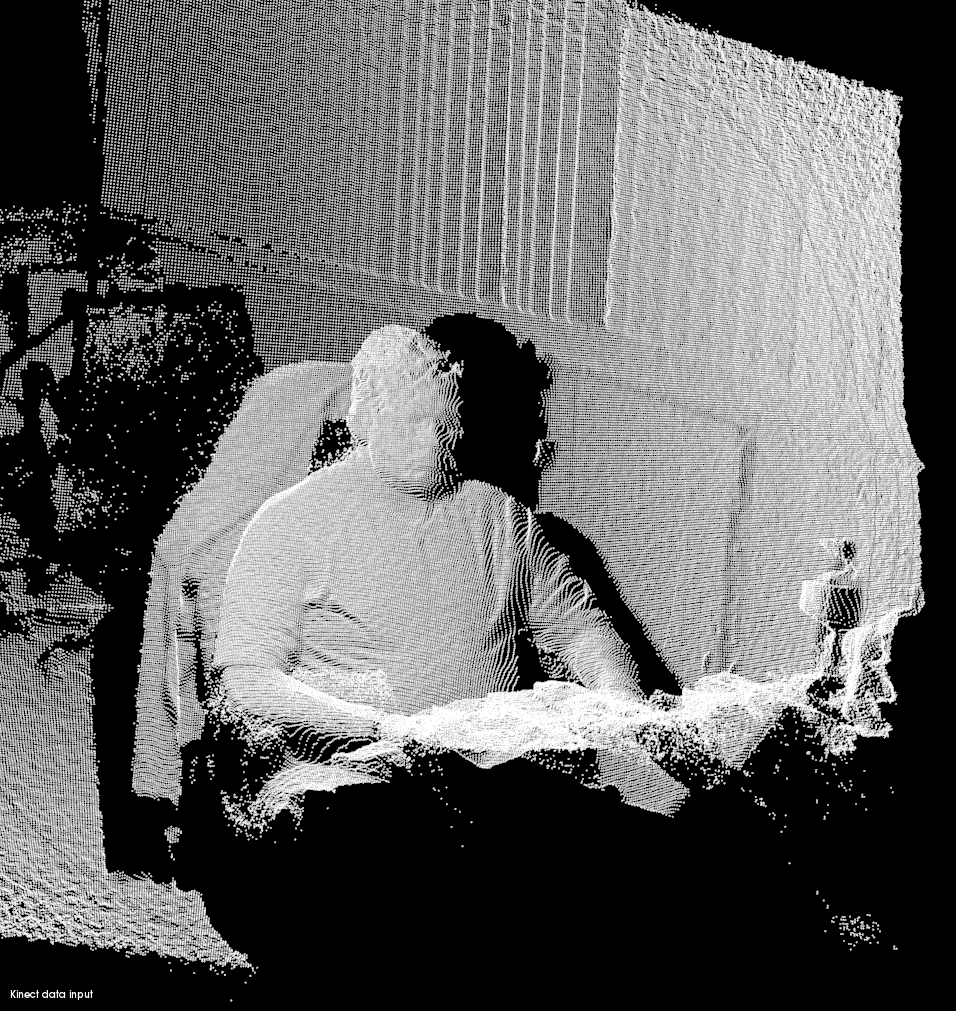
\includegraphics[width=0.45\textwidth]{02Desarrollo/Preprocesamiento/imagenes/downSampleA.png}
        	}
	        \subfloat[
	        \label{fig:FiltroDensidadB}]{%
	        	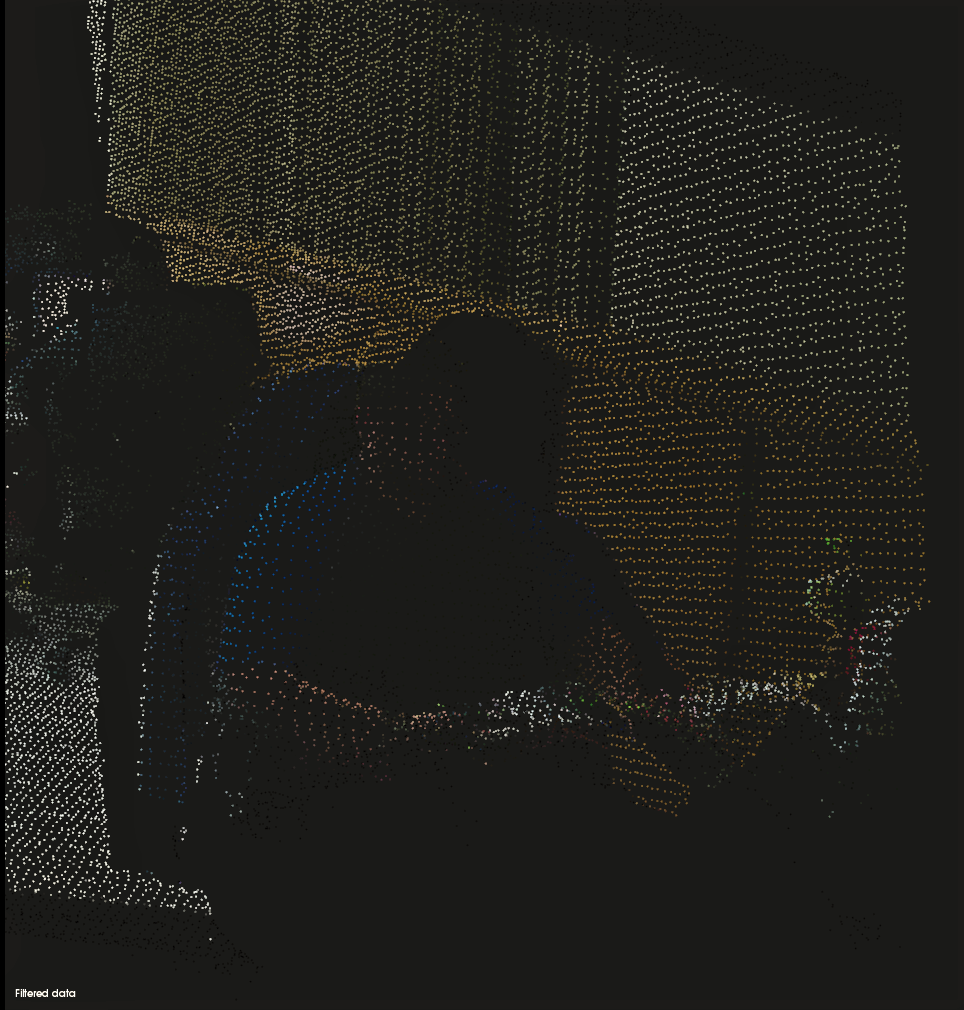
\includegraphics[width=0.45\textwidth]{02Desarrollo/Preprocesamiento/imagenes/downSampleB.png}
	        }
        	\caption[Filtro de densidad de puntos.]{Filtro de densidad de puntos, (a) Nube de puntos obtenida del sensor Kinect, (b) Nube de puntos luego del filtrado de densidad.} 
        	\label{fig:FiltroDensidad}
        \end{figure}
        
        
%        \begin{figure}[!htb] 
%            \centering
%            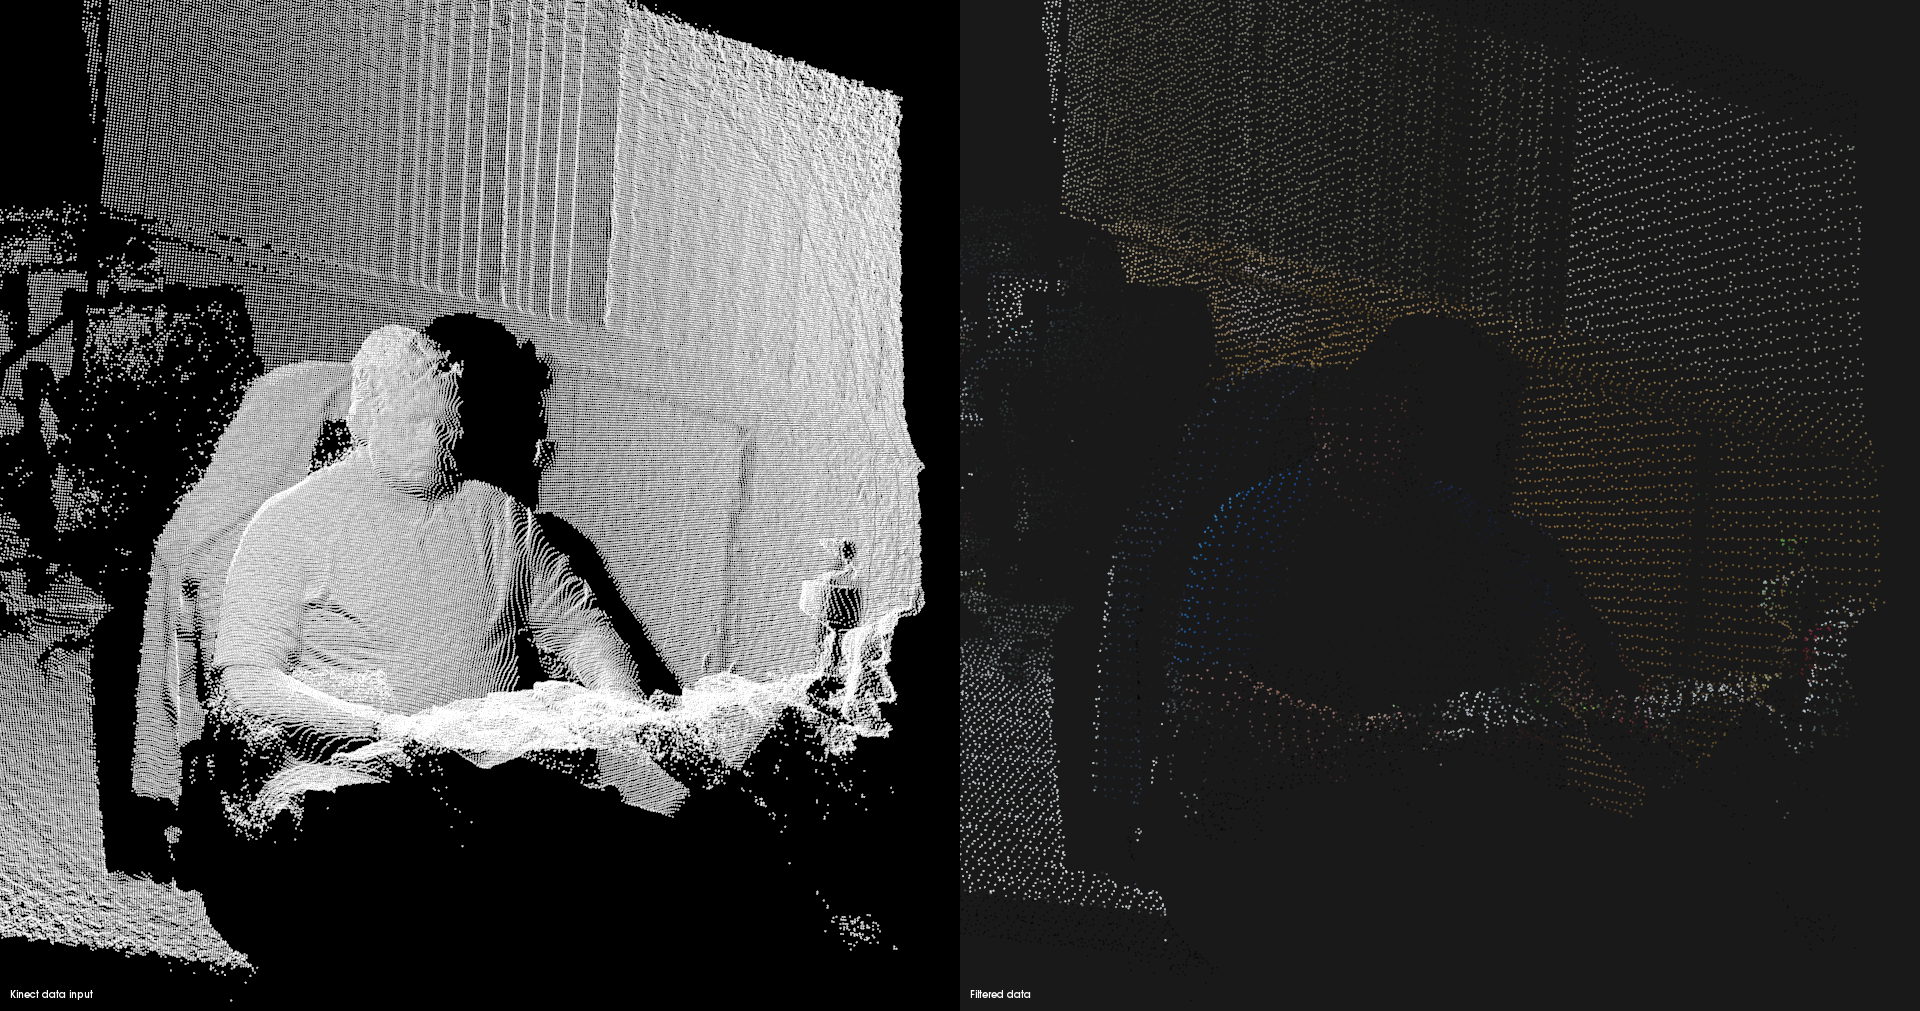
\includegraphics[width=1\textwidth]{02Desarrollo/Preprocesamiento/imagenes/screenshot-1521094833.png}
%            \caption{(izq.)nube de puntos obtenida del sensor Kinect (der.)Nube de puntos luego del filtrado de densidad} 
%            \label{fig:FiltroDensidad}
%        \end{figure}
%        
    \subsection{Operación Resta}
    
        Para detectar los objetos se propuso realizar una comparación entre dos nubes de puntos como se muestra en la figura \ref{fig:resta}, en la figura \ref{fig:restaA}, se muestra la nube que representa los puntos de una escena con la cual no se va a interactuar ni cambiar de lugar ningún objeto, en la figura \ref{fig:restaB}, se muestra la nueva nube de puntos captada con los objetos a representar. Al comparar las nubes de puntos la operación resta muestra los cambios entre la escena estática y la actual, resaltando solo los objetos de interés, como se muestra en la figura \ref{fig:restaC}. 
        Esta operación es similar a la operación resta entre imágenes, con la diferencia de que se realiza en tres dimensiones sobre nubes de puntos. \\
        
        
        \begin{figure}[!htb] 
        	\centering
        	\subfloat[
        	\label{fig:restaA}]{%
        		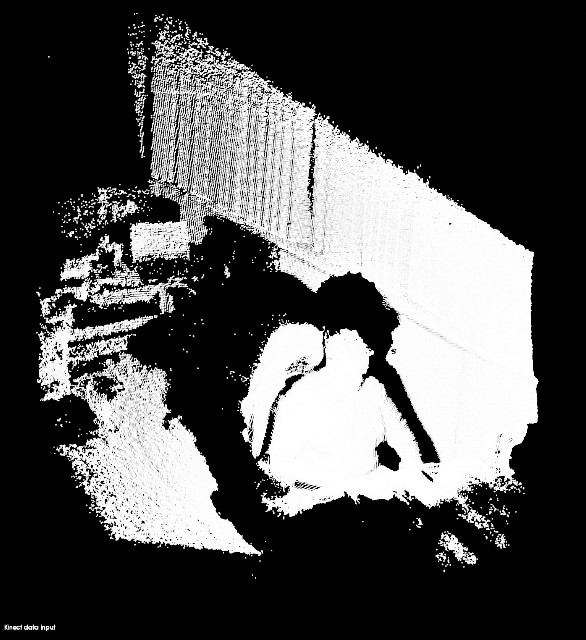
\includegraphics[width=0.33\textwidth]{02Desarrollo/Preprocesamiento/imagenes/andA.jpg}
        	}
        	\subfloat[
        	\label{fig:restaB}]{%
        		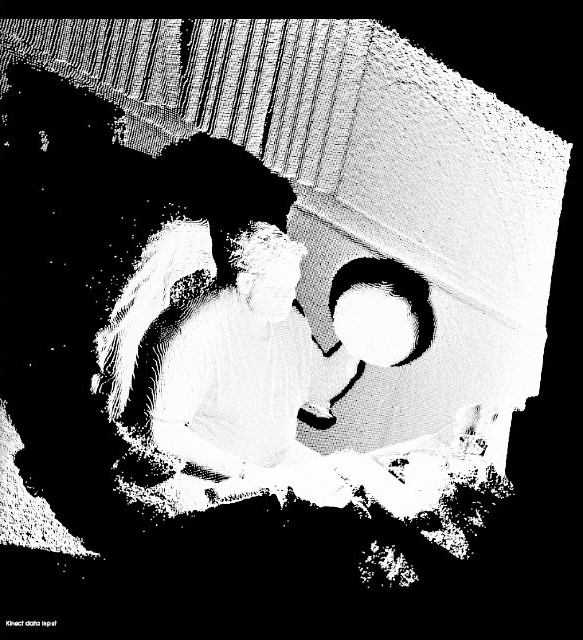
\includegraphics[width=0.33\textwidth]{02Desarrollo/Preprocesamiento/imagenes/andB.jpg}
        	}
	        \subfloat[
		    \label{fig:restaC}]{%
		    	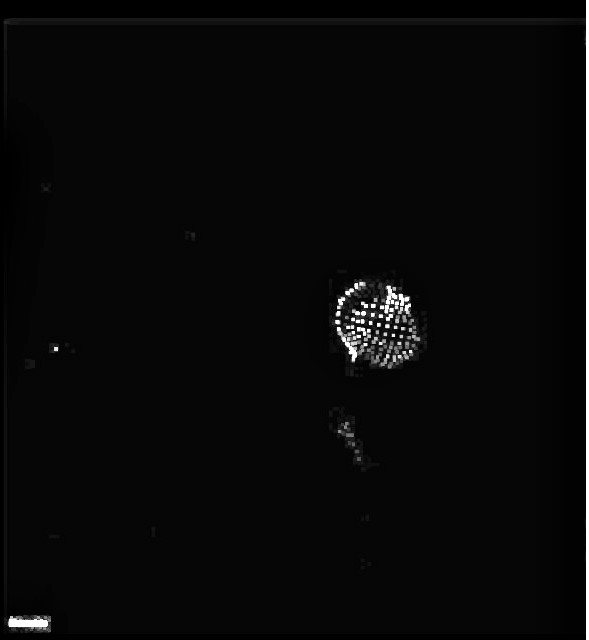
\includegraphics[width=0.33\textwidth]{02Desarrollo/Preprocesamiento/imagenes/andC.jpg}
			}
        	\caption[Operación resta.]{Operación resta, (a) Escena estática, (b) Escena nueva con objetos., (c) Nube de puntos luego de la operación resta.} 
        	\label{fig:resta}
        \end{figure}
        
%        \begin{figure}[!htb]
%            \centering
%            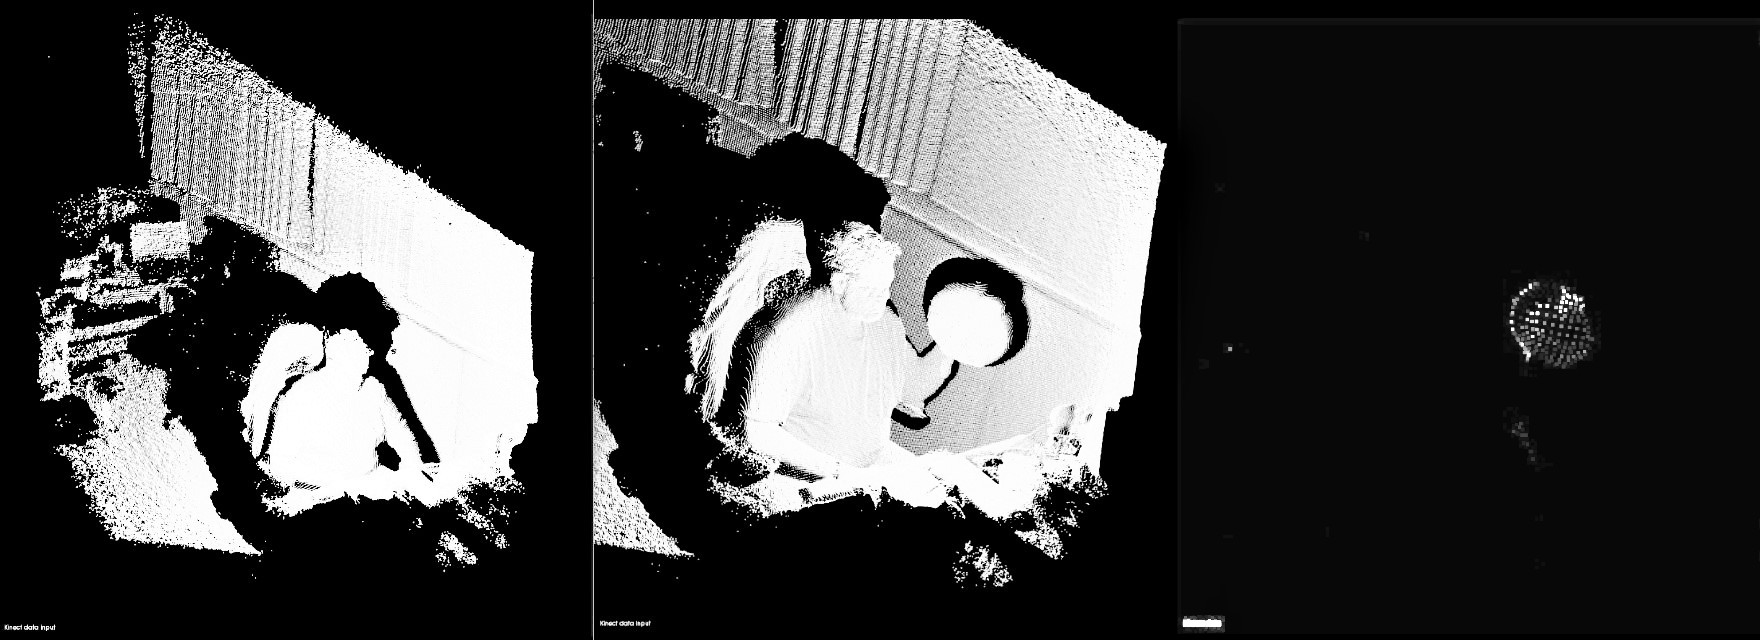
\includegraphics[width=1\textwidth]{02Desarrollo/Preprocesamiento/imagenes/and.jpg}
%            \caption{(izq.)Escena estática, (centro) Escena nueva con objetos, (der.) nube de puntos luego de la operación resta.} \label{fig:resta}
%        \end{figure}
            
    \subsection{Agrupamiento}
    
        Teniendo la nube de puntos con únicamente los puntos de los objetos que nos interesan, ahora lo que se hace es separar en nubes cada objeto. Para esta tarea se realiza una operación llamada Clustering, que traducida se puede interpretar como agrupar, en este caso se usa para agrupar los puntos cercanos.\\
        
        EL proceso de agrupamiento se muestra en el \gls{algoritmo} \ref{alg:agupamiento}.        
        \begin{algorithm}
        	\caption{Agrupamiento}
        	\label{alg:agupamiento}
        	\Begin{
        		\While{N contenga puntos}{
        		NN=Nueva nube de puntos\\
        		NN.add(N[0])\\
        		N.remove(N[0])\\
        		\ForEach{P \textbf{in} NN}{
        			\ForEach{p \textbf{in}N}{
        				\If{Distancia de p a P < intervalo}{
        					NN.add(p)
        					N.remove(p)
        					}
        				}
        			}
        		LN.add(NN)
        		}
        	}
        \end{algorithm}
%        \lstset {language=[Sharp]C}
%        \begin{lstlisting}
%while(N contenga puntos){
%    NN = nueva nube de puntos
%    NN.add(N[0])
%    N.remove(N[0])
%    foreach(P in NN){
%        foreach(p in N) {
%            if( Distancia de p a P < intervalo){
%                NN.add(p)
%                N.remove(p)
%            }
%        }
%    }
%    LN.add(NN)
%}
%return LN
%        \end{lstlisting}
        
        Donde:
        \begin{itemize}
            \item P y p son puntos\\
            \item N es la nube de puntos\\
            \item NN es una nueva nube de puntos que contiene un objeto\\
        \end{itemize}  
        Al final se obtiene un arreglo de nubes y cada nube contiene los datos de un solo objeto, y así trabajar con cada objeto por separado.\\
        
        
        
%        \begin{figure}[!htb]
%            \centering
%            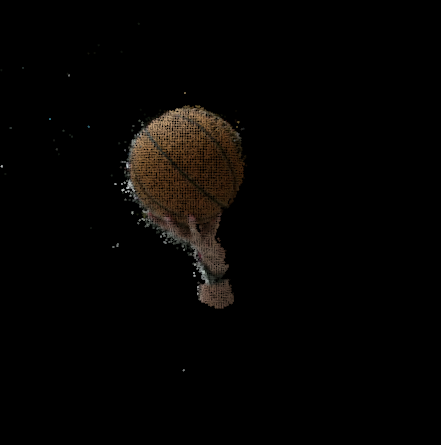
\includegraphics[width=0.7\textwidth]{02Desarrollo/Preprocesamiento/imagenes/filtro.PNG}
%            \caption{Nube de puntos luego del agrupamiento} 
%            \label{fig:Cluster}
%        \end{figure}
            